\documentclass[10pt,a4paper]{article}
\usepackage[utf8]{inputenc}
\usepackage[spanish,es-nodecimaldot]{babel}
\usepackage[margin=1.25cm,top=1.15cm,bottom=1.15cm]{geometry}
\usepackage{graphicx}
\usepackage{booktabs}
\usepackage{tabularx}
\usepackage{amsmath,amssymb}
\usepackage{hyperref}
\usepackage{times}
\usepackage{xcolor}
\usepackage[hypcap=false]{caption}
\usepackage{microtype}

\hypersetup{
    colorlinks=true,
    linkcolor=blue!70!black,
    urlcolor=blue!70!black,
    citecolor=black
}

\graphicspath{{./img/}{../src/img/}}
\captionsetup{font=scriptsize,labelfont=bf,skip=2pt}

\setlength{\parindent}{0pt}
\setlength{\parskip}{2.2pt}
\setlength{\emergencystretch}{2.5em}

\begin{document}


\begin{center}
    {\textbf{\normalsize UNIVERSIDAD TÉCNICA ESTATAL DE QUEVEDO}}\\[0.03cm]
    {\textbf{\small FACULTAD DE CIENCIAS DE LA COMPUTACIÓN -- CARRERA DE SOFTWARE}}\\[0.02cm]
    {\scriptsize \textbf{Aplicaciones Distribuidas (ISR-701) -- SPA 2026--2027 -- Docente: Prof. Gleiston C. Guerrero-Ulloa, PhD}}\\[0.06cm]
    {\textbf{\large EV - Unidad I - Aporte Parte Práctica: TurnoJusto (Turnos Distribuidos)}}\\[0.04cm]
    {\scriptsize \textbf{Estudiante:} MACIAS VÁSQUEZ CÉSAR ABRAHAN \quad|\quad \textbf{Email:} \url{cmaciasv4@uteq.edu.ec} \quad|\quad \textbf{Fecha:} 23/11/2026}\\[0.02cm]
    {\scriptsize \textbf{Repositorio GitHub:} \url{https://github.com/CesarMacias007/AP-U1-MACIAS-CESAR}}
\end{center}
\vspace{-0.25cm}
\hrule
\vspace{0.12cm}

\section{Arquitectura y Ejecución de Escenarios de Prueba (E0 a E6)}

El prototipo \textbf{TurnoJusto} resuelve la entrega ordenada y concurrente de turnos de atención para una agencia municipal mediante un esquema distribuido cliente-servidor sobre sockets TCP en Java 21, compuesto por un Coordinador centralizado (ID 0) y tres ventanillas (V1, V2 y V3, IDs 1, 2 y 3). La comunicación intercambia mensajes JSON delimitados por salto de línea (\texttt{\textbackslash n}) procesados mediante \texttt{BufferedReader} y \texttt{PrintWriter}, garantizando que peticiones consecutivas no se mezclen ni se corten (Requerimiento A2). Todo mensaje incluye autenticación por token (\texttt{UTEQ2026\_SECRETO}) y reloj lógico de Lamport.

\vspace{-0.1cm}
\begin{table}[!ht]
\centering
\scriptsize
\renewcommand{\arraystretch}{0.92}
\begin{tabularx}{\textwidth}{c p{3.1cm} p{1.3cm} p{5.1cm} X}
\toprule
\textbf{Esc.} & \textbf{Objetivo Evaluado} & \textbf{Captura} & \textbf{Evidencia Observada en Consola} & \textbf{Interpretación Técnica} \\
\midrule
\textbf{E0} & Desconexión de red al inicio. & Fig.~\ref{fig:e0_red} & \texttt{Get-NetAdapter}: adaptadores \texttt{Ethernet} y \texttt{Ethernet 2} en estado \texttt{Disabled}. & Cumplimiento estricto de la regla R1 sin conexiones de red durante la prueba. \\
\textbf{E1} & Operación normal de turnos y llamadas. & Fig.~\ref{fig:e1_coord}, \ref{fig:e1_v1} & V1, V2 y V3 reciben turnos 1, 2 y 3; V1 recibe 4; V2 y V3 llaman a turnos 1 y 2 en orden. & Asignación secuencial sin saltos y atención FIFO. El comando \texttt{estado} es coherente. \\
\textbf{E2} & Cupo agotado y autenticación por token. & Fig.~\ref{fig:e1_coord}, \ref{fig:e1_v1} & Solicitud 11 rechazada por cupo agotado. Orden \texttt{token\_malo} rechazada y registrada. & El coordinador valida atómicamente el cupo y rechaza peticiones no autorizadas. \\
\textbf{E3} & Carga concurrente simultánea (30 hilos). & Fig.~\ref{fig:e3_carga}, \ref{fig:e3_inseguro} & Modo normal: 10 asignados únicos $[1..10]$, 20 rechazados. Modo inseguro: colisiones. & La exclusión mutua protege la sección crítica ante ráfagas simultáneas. \\
\textbf{E4} & Detección de caída y retorno de ventanilla. & Fig.~\ref{fig:e4_coord} & Cierre de V3: a los 6\,s se marca \texttt{CAIDA (L=16)}. Al reabrir V3: marcada \texttt{ACTIVA (L=17)}. & Latidos periódicos cada 2\,s con timeout a los 6\,s ($3 \times$ período) tolerando jitter. \\
\textbf{E5} & Resiliencia ante coordinador caído. & Logs y consola & Coordinador detenido; V1 aborta operación y muestra alerta de fallo de conexión. & Priorización de consistencia estricta (modelo CP en CAP) sin emitir números erróneos. \\
\textbf{E6} & Orden total y causalidad con Lamport. & Fig.~\ref{fig:e6_lamport} & Programa \texttt{OrdenTotal}: eventos ordenados por $(L, \text{ID})$ preservando causalidad. & Garantía de la relación \textit{happened-before} ($a \to b \Rightarrow L(a) < L(b)$) en mensajes de red. \\
\bottomrule
\end{tabularx}
\caption{Matriz de trazabilidad y verificación de escenarios requeridos (E0 a E6).}
\label{tab:matriz_escenarios}
\end{table}
\vspace{-0.25cm}

\begin{center}
    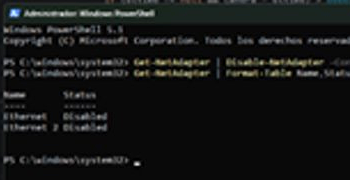
\includegraphics[width=0.72\textwidth,height=3.4cm,keepaspectratio]{fig_e0.png}
    \captionof{figure}{Escenario E0: Desconexión de interfaces físicas y lógicas de red (\texttt{Ethernet} y \texttt{Ethernet 2} en estado \texttt{Disabled}).}
    \label{fig:e0_red}
\end{center}
\vspace{-0.25cm}

\begin{center}
\begin{minipage}{0.49\textwidth}
    \centering
    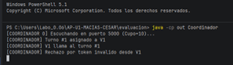
\includegraphics[width=\textwidth,height=2.8cm,keepaspectratio]{fig_e1_coord.png}
    \captionof{figure}{Escenarios E1 y E2: Servidor Coordinador procesando turnos, cupo agotado y token inválido.}
    \label{fig:e1_coord}
\end{minipage}
\hfill
\begin{minipage}{0.49\textwidth}
    \centering
    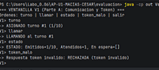
\includegraphics[width=\textwidth,height=2.8cm,keepaspectratio]{fig_e1_v1.png}
    \captionof{figure}{Escenarios E1 y E2: Cliente Ventanilla 1 con asignación, consulta de estado y llamadas.}
    \label{fig:e1_v1}
\end{minipage}
\end{center}

\clearpage


\begin{center}
    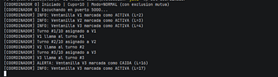
\includegraphics[width=0.78\textwidth,height=3.0cm,keepaspectratio]{fig_e4.png}
    \captionof{figure}{Escenario E4: Detección automática de caída de Ventanilla 3 tras expirar el temporizador de 6\,s (\texttt{TIMEOUT\_CAIDA\_MS}) con $L=16$, y posterior reactivación inmediata al recibir su primer latido con $L=17$.}
    \label{fig:e4_coord}
\end{center}
\vspace{-0.15cm}

\section{Cifras y Análisis Comparativo de la Prueba de Carga Concurrente (E3)}

Para evaluar el control de concurrencia bajo alta demanda, se ejecutó \texttt{PruebaCarga.java}, el cual lanza 30 solicitudes \texttt{TURNO} concurrentes (10 hilos simultáneos por cada una de las 3 ventanillas) sincronizados en el arranque mediante una barrera cíclica (\texttt{CyclicBarrier}) hacia el coordinador con cupo de 10 turnos. Se comparó el \textbf{Modo Normal} (con exclusión mutua mediante cerrojo intrínseco \texttt{synchronized}) frente al \textbf{Modo Inseguro} (\texttt{-inseguro}), obteniéndose los resultados cuantitativos detallados en la Tabla~\ref{tab:cifras_e3}.

\vspace{-0.1cm}
\begin{table}[!ht]
\centering
\small
\renewcommand{\arraystretch}{0.92}
\begin{tabularx}{0.95\textwidth}{X c c}
\toprule
\textbf{Métrica de Evaluación de Concurrencia} & \textbf{Modo Normal (Exclusión Mutua)} & \textbf{Modo Inseguro (\texttt{-inseguro})} \\
\midrule
Total de solicitudes concurrentes lanzadas & 30 hilos & 30 hilos \\
Solicitudes asignadas con éxito (\texttt{ASIGNADO}) & \textbf{10} (Exactamente igual al cupo) & Variable ($> 10$, sobre-emisión de cupo) \\
Solicitudes rechazadas por cupo (\texttt{RECHAZADA}) & \textbf{20} & Variable ($< 20$, rechazos tardíos) \\
Cantidad de números únicos entregados & \textbf{10 distintos} ($[1, 2, 3, 4, 5, 6, 7, 8, 9, 10]$) & Menor a asignados (colisiones y duplicados) \\
Turnos emitidos reportados por el coordinador & \textbf{10} / Cupo: 10 & Estado corrupto ($> 10$ por desfase de lectura) \\
Respeto de exclusión mutua y atomicidad & Garantizado por monitor intrínseco & Violado por retardo artificial de 50\,ms \\
\bottomrule
\end{tabularx}
\caption{Resultados cuantitativos de la prueba de carga concurrente con 30 peticiones simultáneas.}
\label{tab:cifras_e3}
\end{table}
\vspace{-0.25cm}

\begin{center}
\begin{minipage}{0.49\textwidth}
    \centering
    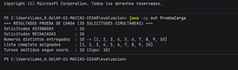
\includegraphics[width=\textwidth,height=2.7cm,keepaspectratio]{fig_e3_carga.png}
    \captionof{figure}{\texttt{PruebaCarga} (Normal): 10 turnos únicos asignados $[1..10]$ y 20 rechazados por cupo.}
    \label{fig:e3_carga}
\end{minipage}
\hfill
\begin{minipage}{0.49\textwidth}
    \centering
    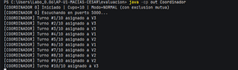
\includegraphics[width=\textwidth,height=2.7cm,keepaspectratio]{fig_e3_inseguro.png}
    \captionof{figure}{Coordinador (Inseguro): colisiones de turnos y sobre-emisión por condiciones de carrera.}
    \label{fig:e3_inseguro}
\end{minipage}
\end{center}
\vspace{-0.2cm}

\textbf{Interpretación técnica de los resultados de E3:} Como se comprueba en las Figuras~\ref{fig:e3_carga} y \ref{fig:e3_inseguro}, en el modo normal el monitor sincronizado (\texttt{synchronized(lockTurnos)}) encapsula la consulta del límite, el incremento del contador y el encolamiento en una operación indivisible. En cambio, en el modo \texttt{-inseguro}, la separación entre la lectura y la actualización junto con la pausa de 50\,ms permite que varios hilos concurrentes lean en paralelo el mismo valor previo del contador antes de actualizarlo, generando colisiones numéricas y superando el cupo fijado de 10.

\section{Relojes Lógicos de Lamport y Verificación de Causalidad (E6)}

Cada proceso mantiene una instancia de \texttt{RelojLamport}. Antes de registrar un evento local o enviar un mensaje por la red, el proceso incrementa su reloj local: $L \leftarrow L + 1$. Al recibir un mensaje con marca $L_{remoto}$, el receptor sincroniza su reloj aplicando la regla de Lamport: $L \leftarrow \max(L, L_{remoto}) + 1$. Cada evento se escribe en el archivo \texttt{logs/<proceso>.log} con formato \texttt{lamport;id\_proceso;evento;detalle}. El programa \texttt{OrdenTotal.java} combina los registros de los cuatro procesos (\texttt{coordinador.log}, \texttt{ventanilla\_1.log}, \texttt{ventanilla\_2.log} y \texttt{ventanilla\_3.log}) en \texttt{logs/orden\_total.log}, ordenándolos ascendentemente por $L$ y desempatando por el identificador del proceso.

\vspace{-0.15cm}
\begin{center}
    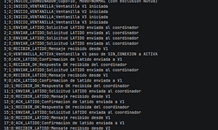
\includegraphics[width=0.68\textwidth,height=3.4cm,keepaspectratio]{fig_e6_lamport.png}
    \captionof{figure}{Visualización del archivo unificado \texttt{logs/orden\_total.log} generado por \texttt{OrdenTotal}, confirmando la ordenación estricta por par $(L, \text{ID})$ y el respeto a la causalidad distribuida.}
    \label{fig:e6_lamport}
\end{center}
\vspace{-0.15cm}

A partir del archivo \texttt{logs/orden\_total.log}, se extraen los siguientes \textbf{dos pares causales reales} que demuestran el respeto estricto a la relación \textit{happened-before} ($a \to b \implies L(a) < L(b)$):
\begin{enumerate}\setlength{\itemsep}{1pt}\setlength{\parskip}{0pt}\setlength{\parsep}{0pt}
    \item \textbf{Par Causal 1 (Solicitud y Recepción de Turno V1 $\to$ Coordinador)}:
    \begin{itemize}\setlength{\itemsep}{0pt}\setlength{\parskip}{0pt}
        \item \textit{Evento emisor ($e_1$):} \texttt{127;1;ENVIAR\_TURNO;Solicitud TURNO enviada al coordinador} (V1, $L(e_1) = 127$).
        \item \textit{Evento receptor ($e_2$):} \texttt{128;0;RECIBIR\_TURNO;Mensaje recibido desde V1} (Coordinador 0, $L(e_2) = 128$).
        \item \textit{Verificación causal:} Dado que $e_1$ causa $e_2$ por envío de mensaje, se cumple $L(e_1) < L(e_2)$ ($127 < 128$). El coordinador actualiza su reloj a $\max(L_{local}, 127) + 1 = 128$.
    \end{itemize}
    \item \textbf{Par Causal 2 (Solicitud y Recepción de Turno V2 $\to$ Coordinador)}:
    \begin{itemize}\setlength{\itemsep}{0pt}\setlength{\parskip}{0pt}
        \item \textit{Evento emisor ($e_3$):} \texttt{205;2;ENVIAR\_TURNO;Solicitud TURNO enviada al coordinador} (V2, $L(e_3) = 205$).
        \item \textit{Evento receptor ($e_4$):} \texttt{206;0;RECIBIR\_TURNO;Mensaje recibido desde V2} (Coordinador 0, $L(e_4) = 206$).
        \item \textit{Verificación causal:} Se cumple $e_3 \to e_4$ con $L(e_3) < L(e_4)$ ($205 < 206$), garantizando que el evento de envío antecede siempre a su recepción en el orden total.
    \end{itemize}
\end{enumerate}

\section{Respuestas a las Preguntas de Análisis}

\subsection*{1. En E3, ¿por qué el modo -inseguro entregó números repetidos o más turnos que el cupo? ¿Qué mecanismo de su código evita ese error en el modo normal y qué costo tiene?}
En el modo \texttt{-inseguro}, el código del coordinador separa la verificación y lectura del contador de turnos de su incremento mediante una pausa de 50 milisegundos:
\vspace{-0.1cm}
{\footnotesize
\begin{verbatim}
int actual = emitidos;
if (actual >= cupo) { /* rechazo */ }
Thread.sleep(50); // Pausa artificial fuera de seccion sincronizada
emitidos = actual + 1;
\end{verbatim}
}
\vspace{-0.15cm}
Al someter el sistema a 30 peticiones concurrentes simultáneas lanzadas por los hilos de \texttt{PruebaCarga}, se desata una \textbf{condición de carrera} (\textit{race condition}). Múltiples hilos concurrentes leen la variable \texttt{actual} durante la ventana de 50\,ms observando el mismo valor (por ejemplo, con \texttt{emitidos=2}, varios hilos leen 2). Al despertar de la pausa, cada hilo calcula \texttt{actual + 1 = 3} y lo asigna, provocando la entrega de turnos con el mismo identificador. Asimismo, varios hilos traspasan la comprobación de cupo (\texttt{actual >= cupo}) simultáneamente antes de que cualquiera actualice \texttt{emitidos}, emitiendo más turnos que el cupo fijado de 10.

En el modo normal, este fallo se previene aplicando \textbf{exclusión mutua} mediante el monitor intrínseco de Java:
\vspace{-0.1cm}
{\footnotesize
\begin{verbatim}
synchronized (lockTurnos) {
    if (emitidos >= cupo) return respuestaRechazo();
    emitidos++;
    colaEspera.add(emitidos);
    return respuestaAsignado(emitidos);
}
\end{verbatim}
}
\vspace{-0.15cm}
\textbf{Costo asociado:} La exclusión mutua impone la \textbf{serialización obligatoria} de las peticiones concurrentes. Esto provoca contención de bloqueo (\textit{lock contention}), un aumento en la latencia de respuesta bajo alta carga y establece un cuello de botella centralizado que restringe el rendimiento máximo (\textit{throughput}) de transacciones por segundo del coordinador.

\subsection*{2. En E5, ¿qué priorizó su sistema, la consistencia de la numeración o la disponibilidad de las ventanillas? Relaciónelo con el teorema CAP. Si cada ventanilla, sin coordinador, entregara números propios con un prefijo (por ejemplo, V2-015), ¿qué propiedad de la Parte B se conservaría y cuál se perdería?}
En el escenario E5, el sistema priorizó de forma estricta la \textbf{Consistencia (C)} sobre la \textbf{Disponibilidad (A)}, posicionándose como un diseño \textbf{CP} bajo el Teorema CAP. Cuando el coordinador cae, la ventanilla detecta la interrupción mediante una excepción \texttt{IOException} producida por el cierre del socket o el vencimiento del timeout de conexión fijado en 3 segundos. En lugar de emitir turnos autónomamente, el cliente aborta la operación, registra \texttt{ERROR\_COORDINADOR\_CAIDO} y notifica en consola: \textit{``ERROR: Coordinador caído. Operación cancelada para mantener consistencia''}. El sistema prefiere denegar el servicio antes que generar inconsistencias globales en la numeración.

Si cada ventanilla entregara turnos propios con prefijo (\texttt{V1-xxx}, \texttt{V2-xxx}, \texttt{V3-xxx}) ante la caída del coordinador (mutando hacia un modelo \textbf{AP}):
\begin{itemize}\setlength{\itemsep}{0pt}\setlength{\parskip}{0pt}
    \item \textbf{Propiedad conservada:} Se mantendría la \textit{unicidad de los identificadores de turno} (ninguna persona recibiría un código idéntico porque los espacios de prefijo son disjuntos) y la \textit{disponibilidad operativa} local de cada ventanilla sin depender del nodo central.
    \item \textbf{Propiedad perdida:} Se perdería la \textit{secuencia consecutiva global sin saltos} ($1, 2, 3, \dots, N$) y el \textit{control del cupo máximo global de la jornada} (Requerimiento B1). Al carecer de sincronización centralizada, las ventanillas desconocerían cuántos turnos han emitido las demás, superando inevitablemente el cupo total de 10 personas e impidiendo establecer un orden de llamada equitativo e intercalado FIFO.
\end{itemize}

\clearpage

\subsection*{3. Su coordinador es un punto único de fallo. ¿Qué mecanismo de la Unidad I usaría para que el sistema siga funcionando si el coordinador cae, y qué problema nuevo aparecería con el último número emitido si hubiera varias réplicas?}
Para eliminar el coordinador como \textbf{punto único de fallo} (\textit{Single Point of Failure} -- SPOF), se emplearía el mecanismo de \textbf{Replicación con Elección de Líder} estudiado en la Unidad I (como el \textit{Algoritmo de Elección del Matón / Bully} o esquemas de réplica primaria con respaldos pasivos/activos). En esta configuración, las réplicas monitorean periódicamente al coordinador principal mediante latidos. Si el líder no responde durante el intervalo fijado, las réplicas inician una elección distribuida para promover a una de ellas como nuevo coordinador activo.

\textbf{Nuevo problema con réplicas:} El problema de \textbf{Consenso Distribuido y Consistencia del Estado}. Para que el nuevo líder retome la asignación sin fallas, debe conocer con precisión el último turno emitido (\texttt{emitidos}) y la composición de la \texttt{colaEspera}. Si el coordinador líder original asignó un turno pero cayó antes de que esa actualización se propagara sincrónicamente a los respaldos, la nueva réplica promovida podría reasignar el mismo número de turno o perder clientes en espera. Resolver este dilema exige implementar protocolos de replicación atómica (ej. commit en dos fases o consenso tipo Raft/Paxos), lo cual penaliza la latencia de cada asignación ordinaria.

\subsection*{4. ¿Qué falacia de la computación distribuida tuvo en cuenta al fijar los tiempos de 2 y 6 segundos? ¿Qué pasaría en su sistema si la red tuviera una latencia de 7 segundos?}
Al establecer los tiempos en 2 segundos para el envío de latidos periódicos (\texttt{INTERVALO\_LATIDO\_MS}) y 6 segundos para el umbral de detección de caída (\texttt{TIMEOUT\_CAIDA\_MS}), se tuvieron presentes de manera explícita las falacias \textbf{``La latencia es cero''} y \textbf{``La red es confiable''}. En un entorno distribuido real, los retardos de enrutamiento y la contención de buffers hacen imposible garantizar entrega instantánea. El umbral de 6 segundos proporciona un margen de tolerancia equivalente a $3 \times$ el intervalo de latido, evitando declarar erróneamente como caída a una ventanilla que solo experimenta congestión transitoria o retrasos menores de transmisión.

Si la red sufriera una latencia persistente de 7 segundos:
\begin{itemize}
    \item \textbf{Falsos positivos masivos de caída:} Cada paquete de latido tardaría 7 segundos en alcanzar el socket del coordinador. Como el evaluador compara $(ahora - \text{ultimoLatido}) > 6\,000\,\text{ms}$, el coordinador marcaría permanentemente a todas las ventanillas en estado \texttt{CAIDA}, a pesar de que los procesos están perfectamente operativos. Al llegar tardíamente los latidos acumulados, el coordinador entraría en un ciclo inestable y oscilatorio entre estados \texttt{ACTIVA} y \texttt{CAIDA}.
    \item \textbf{Fallo por timeout en clientes:} En \texttt{Ventanilla.java}, el tiempo de espera de conexión y socket (\texttt{setSoTimeout}) está calibrado en 3 segundos (3\,000\,ms). Con una latencia de 7\,s, toda solicitud (\texttt{TURNO}, \texttt{LLAMAR}, \texttt{ESTADO} o \texttt{LATIDO}) expirará por \texttt{SocketTimeoutException}, provocando que las ventanillas aborten todas las transacciones asumiendo erróneamente la muerte del servidor.
\end{itemize}

\subsection*{5. Limitación concreta identificada en el prototipo actual}
Una limitación relevante del prototipo es la \textbf{ausencia de persistencia durable en almacenamiento secundario}. Toda la información del servicio (\texttt{emitidos}, \texttt{atendidos}, \texttt{colaEspera}) reside exclusivamente en la memoria volátil (RAM) del proceso Coordinador. Ante una terminación inesperada, fallo de alimentación eléctrica o caída del sistema operativo, el estado de la jornada se borra de forma irrecuperable, impidiendo que el sistema reanude su operación sin reiniciar la numeración desde cero o requiriendo mecanismos de \textit{Write-Ahead Logging} (WAL) o base de datos externa.

\vspace{0.4cm}
\hrule
\vspace{0.2cm}
\begin{center}
    \footnotesize \textit{Informe técnico individual del Aporte Práctico de la Unidad I -- Aplicaciones Distribuidas -- Noviembre 2026.}
\end{center}

\end{document}
